\section{Discrete Kalman filter}
\subsection{Problem a}
Here we are to discretize the system in order to use it to design a discretized Kalman filter. For this we need discrete versions of $\bm{A}, \bm{B}, \bm{E}$, and also discrete versions of the covariances of the disturbance $\bm{Q_w}$, and measurement noise $\bm{R_v}$.

The continuous solution of $\bm{x}$ with an input $\bm{u}$ with gain matrix $\bm{B}$, and disturbance $\bm{w}$ with gain matrix $\bm{E}$ is given by:
\begin{equation*}
\bm{x}(t) = e^{\bm{A}t}\bm{x}_0 + \int_0^te^{\bm{A}(t-\tau)}\bm{Bu}(\tau)d\tau + \int_0^te^{\bm{A}(t-\tau)}\bm{Ew}(\tau)d\tau
\end{equation*}
Using the continuous solution, we start it at $t=kT_s$ and stop it at $t=(k+1)T_s$. Here, $T_s = 1/F_s$ and $F_s = 10$ Hz is the sampling frequency. $T_s$ is thus the sampling period. Doing this, we get:
\begin{equation}
\bm{x}[k+1] = e^{\bm{A}T_s}\bm{x}_0 + \int_0^{T_s} e^{\bm{A}\alpha}\bm{Bu}((k+1)T_s -\alpha)d\alpha + \int_0^{T_s} e^{\bm{A}\alpha}\bm{Ew}((k+1)T_s -\alpha)d\alpha \label{x_disc}
\end{equation}

By setting a sampling period $T_s$ that is low enough, $\bm{u}$ and $\bm{w}$ can be seen as approximately constant between the time $t = kT_s$ and $t = (k+1)T_s$, and can be moved outside of our integral. Moving forward, $T_s$ is assumed to be low enough.

\begin{equation}
\bm{x}[k+1] = e^{\bm{A}T_s}\bm{x}_0 + \bm{u}\int_0^{T_s} e^{\bm{A}\alpha}\bm{B}d\alpha + \bm{w}\int_0^{T_s} e^{\bm{A}\alpha}\bm{E}d\alpha \label{x_disc_const}
\end{equation}

The exact discretized system is thus found to be:
\begin{subequations}
\begin{align}
    \dot{\bm{x}}[k+1] =& \ \thickbar{\bm{A}}\bm{x}[k]+\thickbar{\bm{B}}\bm{u}[k] + \thickbar{\bm{w}}[k], \\
    \thickbar{\bm{w}}[k] &= \thickbar{\bm{E}}\bm{w}[k], \label{w_bar} \\
    \thickbar{\bm{A}} &= e^{\bm{A}T_s}, \\
    \thickbar{\bm{B}} &= \int_{0}^{T_s}e^{\bm{A}\alpha}\bm{B}d\alpha \label{B_d}, \\
    \thickbar{\bm{E}} &= \int_{0}^{T_s}e^{\bm{A}\alpha}\bm{E}d\alpha \label{E_d}
\end{align}
\end{subequations}
The notation $\bm{X_d} = \thickbar{\bm{X}}$ is used in MATLAB code.

In MATLAB, they can be found through the
\texttt{[A$_d$\ B$_d$] = c2d(A, B, T$_s$)} function. \\ \texttt{c2d(A, B, T$_s$)} uses the Van Loan's method:
\begin{equation}
exp(
\begin{bmatrix}
\bm{A} & \bm{B} \\
\bm{0} & \bm{0} \\
\end{bmatrix}
T_s) = 
\begin{bmatrix}
\bm{N}_{11} & \bm{N}_{12} \\
\bm{0} & \bm{I} \\
\end{bmatrix}
,\ \thickbar{\bm{A}} = \bm{N}_{11},\  \thickbar{\bm{B}} = \bm{N}_{12}
\end{equation}
Since $\bm{w}$ can be seen as an input with gain matrix $\bm{E}$ of the continuous system, one can replace $\bm{B}$ with $\bm{E}$ in order to find $\thickbar{\bm{E}}$.

In order to find the autocovariance of $\thickbar{\bm{w}}$, we use the following relation where

\begin{equation*}
    \thickbar{\bm{A}}_{\bm{w}}[k,l] = E((\thickbar{\bm{w}}[k]-\bm{m}_{\thickbar{\bm{w}}}[k])(\thickbar{\bm{w}}[l]-\bm{m}_{\thickbar{\bm{w}}}[l])^T)
\end{equation*}
Noting that the means are zero, and inserting the result in \cref{w_bar}, we get:
\begin{align*}
    \thickbar{\bm{A}}_{\bm{w}}[k,l] &=
    E(\thickbar{\bm{E}}\bm{w}[k]\bm{w}[l]^T\thickbar{\bm{E}}^T) \\
    &= \thickbar{\bm{E}}E(\bm{w}[k]\bm{w}[l]^T)\thickbar{\bm{E}}^T \\
    &= \thickbar{\bm{E}}\bm{Q_w}\delta[k,l]\thickbar{\bm{E}}^T \\
    &= \thickbar{\bm{Q}}_{\bm{w}}\delta[k,l]
\end{align*}
Meaning the discretized $\thickbar{\bm{Q}}_{\bm{w}}$ is:
\begin{equation}
\thickbar{\bm{Q}}_{\bm{w}} =\thickbar{\bm{E}}\bm{Q}_{\bm{w}}\thickbar{\bm{E}}^T
\end{equation}
The discretized output of the system is:
\begin{equation*}
\bm{y}[k] = \bm{Cx}[k] + \thickbar{\bm{v}}[k]
\end{equation*}
where $\thickbar{\bm{v}}[k]$ is the averaged measurement noise. We use this as opposed to the direct measurement noise
at time $kT_s$ in order to avoid the exaggeration of sampling continuous time noise into discrete time.
\begin{equation*}
\thickbar{\bm{v}}[k] = \frac{1}{T_s}\int_{0}^{T_s}\bm{v}(kT-\alpha)d\alpha
\end{equation*}
The autocovariance of the noise becomes (again with mean equal to zero):
\begin{align*}
    \thickbar{\bm{A}}_\bm{v}[k, l] &= E(\thickbar{\bm{v}}[k]\thickbar{\bm{v}}[l]^T) \\
    &= \frac{1}{T_s^2}\int_{0}^{T_s}\int_{0}^{T_s}E(\bm{v}(kT_s-\alpha_1)\bm{v}(lT_s-\alpha_2)^T)d\alpha_1d\alpha_2 \\
    &= \frac{1}{T_s^2}\int_{0}^{T_s}\int_{0}^{T_s}\bm{R_v}\delta[k,l]\delta(\alpha_1-\alpha_2)d\alpha_1d\alpha_2 \\
    &= \frac{1}{T_s^2}\int_{0}^{T_s}\bm{R_v}\delta[k,l]d\alpha_1 \\
    &= \frac{1}{T_s}\bm{R_v}\delta[k,l] \\
    &= \thickbar{\bm{R}}_{\bm{v}}\delta[k,l]
\end{align*}
Meaning the discretized $\thickbar{\bm{R}}_{\bm{v}}$ is:
\begin{equation}
\thickbar{\bm{R}}_{\bm{v}} = \frac{\bm{R_v}}{T_s}
\end{equation}

\subsection{Problem b}
The ship system is simulated with a constant rudder $\delta$-input of 0 and only measurement noise turned on. An
estimate of the variance of 
the measurement noise is found by putting the compass output into the MATLAB function {\texttt{var(A)}}. This function
sums the squared distance of the values from the mean and divides this by the total number of values. The variance 
is found to be 0.0020.

\subsection{Problem c}
A discrete Kalman filter is to be designed. It is a discrete observer which performs optimal estimation through
minimizing the mean-square-error $J[k] = tr(\bm{P}[k])$, where
$\bm{P}[k] \triangleq E(\bm{e}[k]\bm{e}[k]^T) = E((\bm{x}[k] - \hat{\bm{x}}[k])(\bm{x}[k] - \hat{\bm{x}}[k])^T)$ is the
covariance matrix of the error between the states and the estimated states.

The estimate is generated in two phases, one guess for $\bm{x}[k]$ before $\bm{y}[k]$ is taken into account, called a
priori (prior observation), and one guess after called a posteriori (post observation).

A priori estimate:
\begin{equation}
\hat{\bm{x}}^-[k] = \thickbar{\bm{A}}\hat{\bm{x}}[k-1]+\thickbar{\bm{B}}\bm{u}[k-1] \label{a_priori_x}
\end{equation}
This is thus an a priori guess of the next $\hat{\bm{x}}[k]$ based on the previous a posteriori value of $\hat{\bm{x}}$ and the value of $\bm{u}$ at time k-1.

A posteriori estimate:
\begin{equation}
\thickbar{\bm{x}}[k] = \hat{\bm{x}}^-[k] + \bm{L}[k](\bm{y}[k] - \bm{C}\hat{\bm{x}}^-[k]) \label{a_posteriori_estimate}
\end{equation}
And this is the update of $\thickbar{\bm{x}}[k]$ based on the a priori value, the measured $\bm{y}[k]$, and the updated Kalman gain $\bm{L}[k]$.

With this, we can also define an a priori error and an a posteriori error, and an a priori and a posteriori covariance matrices. They are respectively:
\begin{align}
\bm{e}^-[k] &= \bm{x}[k] - \hat{\bm{x}}^-[k] \\
\bm{e}[k] &= \bm{x}[k] - \hat{\bm{x}}[k] \\
\bm{P}^-[k] &= E(\hat{\bm{x}}^-[k]\hat{\bm{x}}^-[k]^T) \\
\bm{P}[k] &= E(\hat{\bm{x}}[k]\hat{\bm{x}}[k]^T)
\end{align}

Using this information, we can find update rules for $\bm{P}^-[k], \bm{P}[k]$, and $\bm{L}[k]$. First we find update rules for the a priori and a posteriori error:
\begin{align*}
    \bm{e}^-[k] &= \bm{x}[k]-\hat{\bm{x}}^-[k] \\
                &= \thickbar{\bm{A}}\bm{x}[k-1] + \thickbar{\bm{B}}\bm{u}[k-1] + \thickbar{\bm{w}}[k-1] - (\thickbar{\bm{A}}\hat{\bm{x}}[k-1] + \thickbar{\bm{B}}\bm{u}[k-1]) \\
                &= \thickbar{\bm{A}}\bm{e}[k-1] + \thickbar{\bm{w}}[k-1] \\
    \bm{e}[k]&= \bm{x}[k] -\hat{\bm{x}}[k] \\
             &= \bm{x}[k] - (\bmhat{x}^-[k]+\bm{L}[k](\bm{y}-\bm{C}\bmhat{x}^-[k])) \\
             &= \bm{x}[k] - (\bmhat{x}^-[k]+\bm{L}[k](\bm{C}\bm{x}[k] -\bm{C}\bmhat{x}^-[k]+\bmbar{v}[k])) \\
             &= \bm{e}^-[k] - \bm{L}[k]\bm{C}\bm{e}^-[k]-\bm{L}[k]\bmbar{v}[k]
\end{align*}
The a priori covariance matrix becomes:
\begin{align*}
    \bm{P}^-[k] &= E(\bm{e}^-[k]\bm{e}^-[k]^T) \\
                &= E((\thickbar{\bm{A}}\bm{e}[k-1] + \thickbar{\bm{w}}[k-1])(\thickbar{\bm{A}}\bm{e}[k-1] + \thickbar{\bm{w}}[k-1])^T) \\
                &= \thickbar{\bm{A}}E(\bm{e}[k-1]\bm{e}[k-1]^T)\thickbar{\bm{A}}^T + E(\thickbar{\bm{w}}[k-1]\thickbar{\bm{w}}[k-1]^T)
\end{align*}
The last line follows because $\bm{e}$ and $\bm{w}$ are uncorrelated. This simplifies to
\begin{equation}
\bm{P}^-[k] = \thickbar{\bm{A}}\bm{P}[k-1]\thickbar{\bm{A}}^T + \thickbar{\bm{Q}}_{\bm{w}} \label{a_priori_covariance}
\end{equation}

And the a posteriori covariance matrix becomes:
\begin{align*}
    \bm{P}[k] &= E(\bm{e}[k]\bm{e}[k]^T) \\
              &= E(\ ((\bm{I} - \bm{L}[k]\bm{C})\bm{e}^-[k]+\bm{L}[k])((\bm{I} - \bm{L}[k]\bm{C})\bm{e}^-[k]+\bm{L}[k])^T) \\
              &= (\bm{I} - \bm{L}[k]\bm{C})E(\bm{e}^-[k]\bm{e}^-[k]^T)(\bm{I} - \bm{L}[k]\bm{C})^T + \bm{L}[k]\bmbar{R}_{\bm{v}}\bm{L}[k]^T
\end{align*}
Again, where the last line follows because $\bm{e}^-[k]$ and $\bmbar{v}$ are uncorrelated. The result:
\begin{equation}
              \bm{P}[k] = (\bm{I} - \bm{L}[k]\bm{C})\bm{P}^-[k](\bm{I} - \bm{L}[k]\bm{C})^T + \bm{L}[k]\bmbar{R}_{\bm{v}}\bm{L}[k]^T \label{a_posteriori_covariance}
\end{equation}

Lastly, we can now find the update rule for $\bm{L}[k]$. This is the Kalman gain, and it functions as a gain to $\bm{y}$ and the estimated $\bmhat{y} = \bm{C}\bmhat{x}$. It is selected in order to minimize the error between them. The Kalman gain $\bm{L}[k]$ is found by minimizing the mean-square-error $J[k] = tr(\bm{P}[k])$ with respect to $\bm{L}[k]$, i.e $\frac{\partial tr(\bm{P}[k])}{\partial\bm{L}[k]} = \bm{0}$. The result:
\begin{equation}
\bm{L}[k] = \bm{P}^-[k]\bm{C}^T(\bm{CP}^-[k]\bm{C}^T+\bmbar{R}_{\bm{v}})^{-1} \label{kalman_update}
\end{equation}

And with all that, the Kalman filter can be designed. It performs the following calculations in the following order:
\begin{enumerate}
 \item $\bmhat{x}^-[0]$ and $\bm{P}^-[0]$ are initialized to $E(\bm{x}[0]) = \bm{m}_{\bm{x}_0}$ and $E(\bm{e}^-[0]\bm{e}^-[0]^T) = \mathcal{C}_{\bm{x}_0}$ respectively.
 \item The update of the Kalman gain is performed using  \cref{kalman_update}.
 \item The a posteriori estimate of the states is calculated using  \cref{a_posteriori_estimate}.
 \item The error covariance matrix is updated using  \cref{a_posteriori_covariance}.
 \item The a priori values of $\bmhat{x}^-$ and $\bm{P}^-$ are found for the next time step $k+1$, using \cref{a_priori_x} and \cref{a_priori_covariance}.
 \item Start from step 2 again for the next time step $k+1$.
\end{enumerate}

This was implemented in simulink using zero-order hold blocks to discretize to system by holding the values for each time step, and memory blocks to hold the previous a priori values first initialized in step 1, and updated in step 5 above. The updates were implemented as function blocks, and the updates themselves were thus written as MATLAB functions. These can be seen in \cref{sec:Appendix A}.

\subsection{Problem d}
The Kalman filter gives access to an estimate of the bias to the rubber angle (\cref{fig:5d-estimated_rudder_bias}).  With current disturbance on, this bias became apparent when attempting to steer the ship (Part 3C \cref{fig:3b-psi_and_rudder_w_current}).  However, this bias can now be compensated for by adding the estimated bias as a feedforward term to the rudder input.  The results of using this term, with current disturbances on, is seen in \cref{fig:5d-psi_and_rudder}.  This term removes the steady state error seen previously.

\begin{figure}[ht]
    \centering
    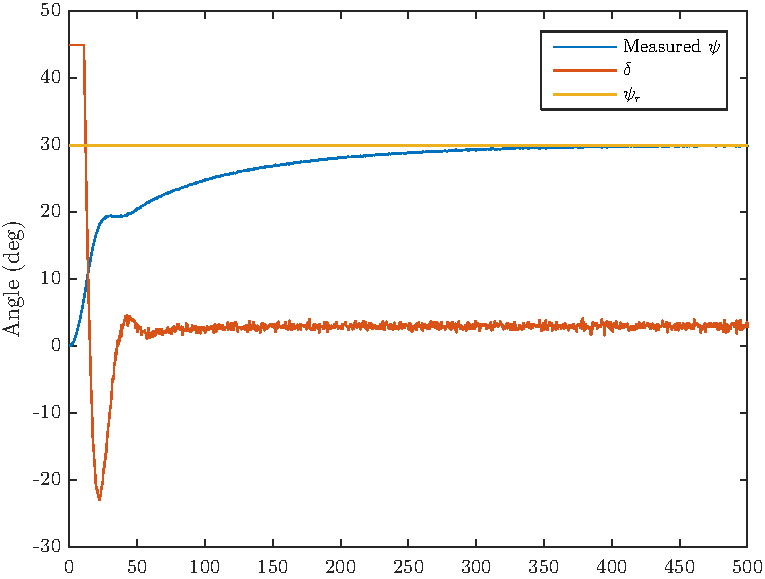
\includegraphics[width=0.5\textwidth]{images/5d-psi_and_rudder}
    \caption{Compass angle, $\psi$, and rudder angle, $\delta$, along the y-axis, plotted against time in the x-axis. Using estimated bias from \cref{fig:5d-estimated_rudder_bias} as feedforward term added to the rudder input. With current disturbance and measurement noise}
    \label{fig:5d-psi_and_rudder}
\end{figure}

\begin{figure}[ht]
    \centering
    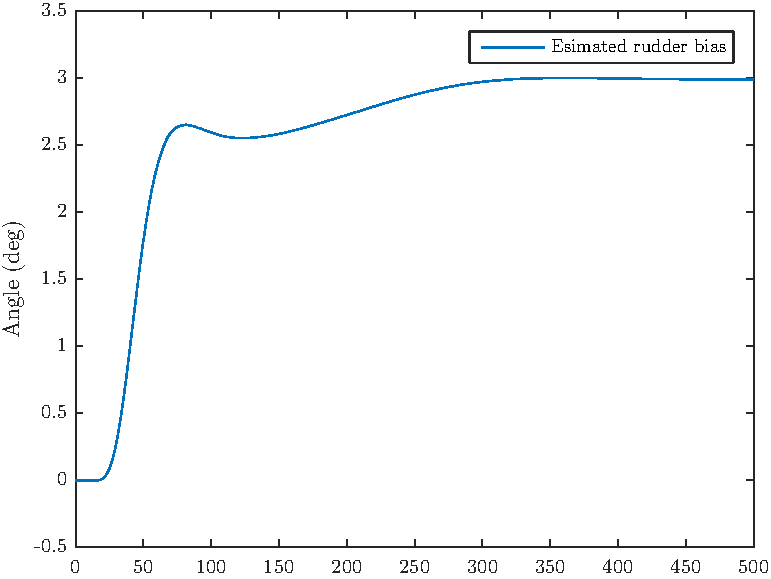
\includegraphics[width=0.5\textwidth]{images/5d-estimated_rudder_bias}
    \caption{Kalman estimated rudder bias over time. With current disturbance and measurement noise}
    \label{fig:5d-estimated_rudder_bias}
\end{figure}

\subsection{Problem e}
The Kalman filter also gives access to a filtered estimate of the compass heading. This reduces the high frequency noise due to the waves on the compass heading. The results of simulating the ship using the filtered estimate for $\psi$ as the input to the controller is shown in \cref{fig:5e-psi_and_rudder}. The estimated compass angle does not have large oscillations compared to the measured compass angle. This leads to reasonable rudder inputs and roughly the same output as the same simulation with the measured compass angle used as feedback (Part3D \cref{fig:3b-psi_and_rudder_w_waves}). Using the inputs from the previous simulation would likely break the rudder or its motor, while these inputs are much more tame and smooth.

\begin{figure}[htp]
    \centering
    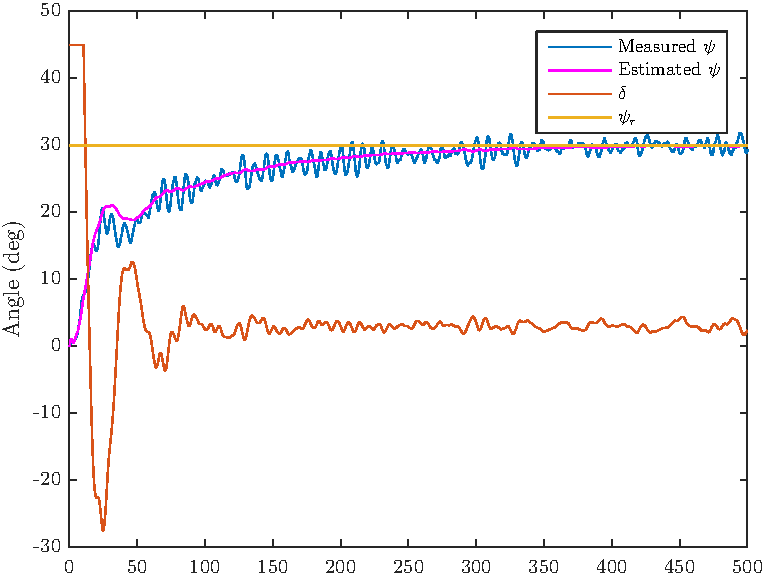
\includegraphics[width=0.5\textwidth]{images/5e-psi_and_rudder}
    \caption{Compass angle, $\psi$, and rudder angle, $\delta$, along the y-axis, plotted against time in the x-axis. Using estimated compass angle as feedback to the controller. With current and wave disturbances and measurement noise}
    \label{fig:5e-psi_and_rudder}
\end{figure}

\begin{figure}[htp]
    \centering
    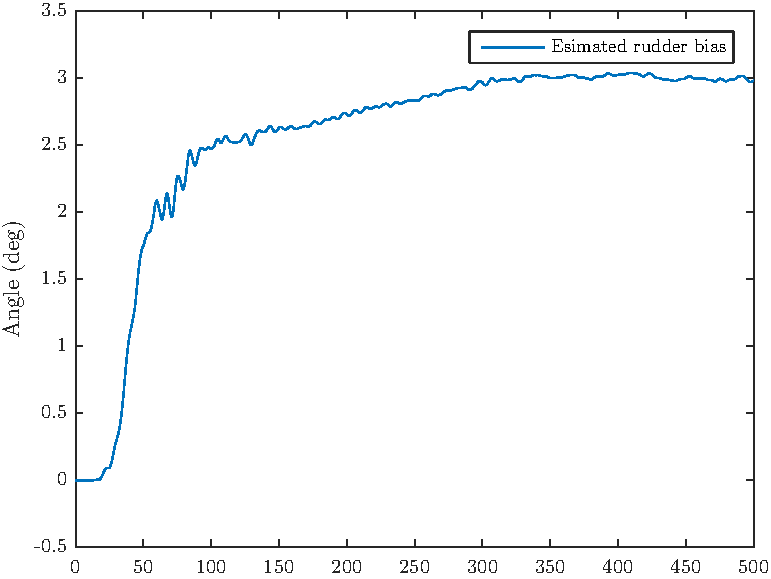
\includegraphics[width=0.5\textwidth]{images/5e-estimated_rudder_bias}
    \caption{Kalman estimated rudder bias over time. With current and wave disturbances and measurement noise}
    \label{fig:5e-estimated_rudder_bias}
\end{figure}

The wave noise estimate follows the pattern of the actual waves, but is quite damped in comparison.  This points to a likely error in the Kalman filter. This error is most likely a mismatched unit, for example degrees instead of radians, and could also explain why the estimated compass angle oscillates around the measured value slightly and the rudder bias oscillates before settling at 3 degrees.  These oscillations seem to be exacerbated by large changes in the measured value, meaning the the Kalman gains are too small, thereby over-prioritizing the current estimated state compared to the new measurements. This can be due to error(s) in the calculation or update of the P matrix, which in turn could be due to the measurement variance or the discretized A or Q matrices.

\begin{figure}[htp]
    \centering
    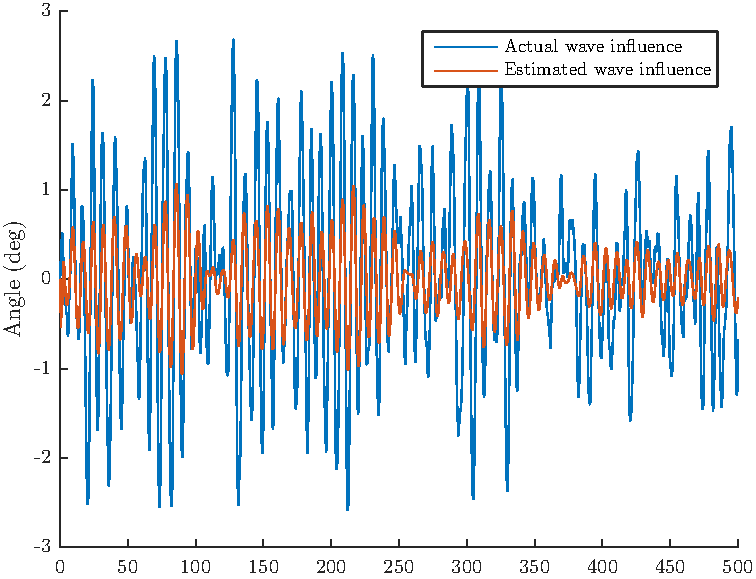
\includegraphics[width=0.5\textwidth]{images/5e-wave_influence}
    \caption{Estimated wave noise versus actual wave noise.}
    \label{fig:5e-wave_influence}
\end{figure}